\chapter{Física sin miedo}

\begin{enpocas}
Vectores, las leyes de Newton aplicadas al dron, por qué el empuje crece con el cuadrado de la
velocidad, qué es la inercia, qué son los marcos de referencia (ENU, NED, cuerpo) y cómo se describe
una rotación. Al final, las ecuaciones del dron en una sola página.
\end{enpocas}

\section{Vectores: flechas con tamaño y dirección}

Muchas cantidades físicas no son solo un número: la velocidad de un dron es ``5~m/s \emph{hacia el
norte}''. Esas cantidades se llaman \textbf{vectores} y se dibujan como flechas. En tres
dimensiones un vector tiene tres componentes, por ejemplo $v = (v_x, v_y, v_z)$. Posición,
velocidad, aceleración, fuerza y velocidad angular son vectores.

\section{Las leyes de Newton aplicadas al dron}

\begin{enumerate}
  \item \textbf{Inercia.} Un cuerpo sigue como está (quieto o moviéndose en línea recta) mientras
        nadie lo empuje. Un dron que avanza y apaga la inclinación sigue avanzando un rato.
  \item \textbf{$F = ma$.} La aceleración es la fuerza total dividida entre la masa. Para el dron:
        \begin{equation}
        m\,\ddot p = \underbrace{T\,R\,e_3}_{\text{empuje}} \;\underbrace{-\,mg\,e_3}_{\text{peso}} \;+\; \underbrace{d(t)}_{\text{viento}}
        \end{equation}
        donde $\ddot p$ es la aceleración, $T$ el empuje total, $R e_3$ la dirección ``arriba'' del
        dron (que cambia si se inclina) y $e_3 = (0,0,1)$ la vertical.
  \item \textbf{Acción y reacción.} La hélice empuja aire hacia abajo y el aire empuja la hélice
        hacia arriba. También explica la guiñada: al hacer girar la hélice, el motor ``empuja'' al
        dron en sentido contrario.
\end{enumerate}

\section{Empuje: el cuadrado de la velocidad}

\begin{figure}[H]
\centering
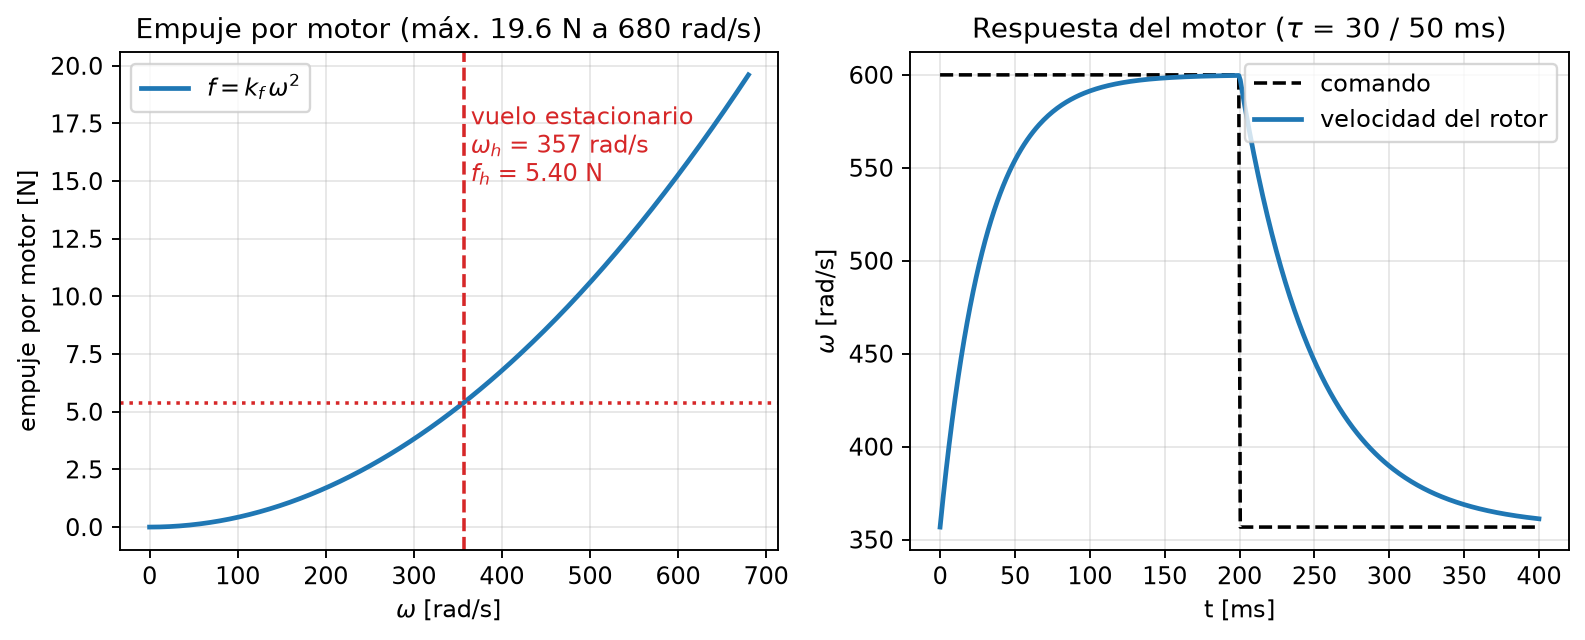
\includegraphics[width=\textwidth]{motor_empuje.png}
\caption{Izquierda: el empuje de un motor del Tarot crece como $\omega^2$. Derecha: el motor no
cambia de velocidad al instante, tarda unos 30--50~ms.}
\label{fig:empuje-fisica}
\end{figure}

El empuje de una hélice es aproximadamente
\begin{equation}
f = k_f\,\omega^2 ,
\end{equation}
con $\omega$ la velocidad de giro en rad/s y $k_f$ una constante que depende de la hélice y del aire.
Que sea cuadrático tiene consecuencias: cerca del vuelo estacionario un pequeño cambio de velocidad da
un cambio de empuje más o menos proporcional, pero no hay una relación lineal en todo el rango, y el
controlador tiene que tenerlo en cuenta (por eso calcula fuerzas y luego saca raíces cuadradas para
obtener velocidades).

Además del empuje, cada hélice produce un \textbf{par de arrastre} (una ``torsión'') proporcional a
su empuje, $k_m f$: es lo que intenta girar al dron al revés de la hélice.

\begin{recuerda}
Los motores no son instantáneos. En el Tarot simulado tardan $\approx$30~ms en acelerar y
$\approx$50~ms en frenar. Ese retardo es parte de lo que hace difícil el control, y tiene un papel
importante en los resultados del control.
\end{recuerda}

\section{Inercia de rotación y par}

Para girar, lo que importa no es la masa sino el \textbf{momento de inercia} $J$: cuánto se resiste
un cuerpo a cambiar su giro. Depende de cómo está repartida la masa: un patinador que encoge los
brazos gira más rápido porque baja su momento de inercia. El dron tiene un momento de inercia para
cada eje (en el Tarot: 0.034, 0.036 y 0.066~kg\,m$^2$; el del eje vertical es mayor porque los
motores están lejos del centro en ese plano).

Lo que hace girar es un \textbf{par} (o torque) $\tau$: una fuerza aplicada a cierta distancia del
centro. Un motor de un brazo que empuja más que el del brazo opuesto produce un par que ladea al dron.
La ``segunda ley de Newton para giros'' es
\begin{equation}
J\,\dot\omega = \tau - \omega\times J\omega .
\end{equation}
El último término es un efecto giroscópico; para entender la idea basta con ``par = inercia por
aceleración angular''.

\section{Marcos de referencia: ¿desde dónde mido?}

Decir ``el dron está en $(3, 5, 10)$'' no significa nada si no se dice desde dónde y con qué ejes.
Eso es un \textbf{marco de referencia}. En este proyecto aparecen tres:

\begin{description}
  \item[Mundo ENU] (Este, Norte, Arriba): fijo al suelo, con origen en el centro del mundo de Gazebo.
        Lo usan Gazebo y ROS.
  \item[Mundo NED] (Norte, Este, Abajo): el mismo lugar, pero con otros ejes. Lo usa la aviación y
        ArduPilot. Pasar de uno a otro es solo cambiar $x\leftrightarrow y$ y el signo de $z$.
  \item[Cuerpo:] pegado al dron y que se mueve con él: \emph{x} al frente, \emph{y} a la izquierda,
        \emph{z} arriba. Los sensores (IMU, cámara, LiDAR) miden en este marco.
\end{description}

\begin{figure}[H]
\centering
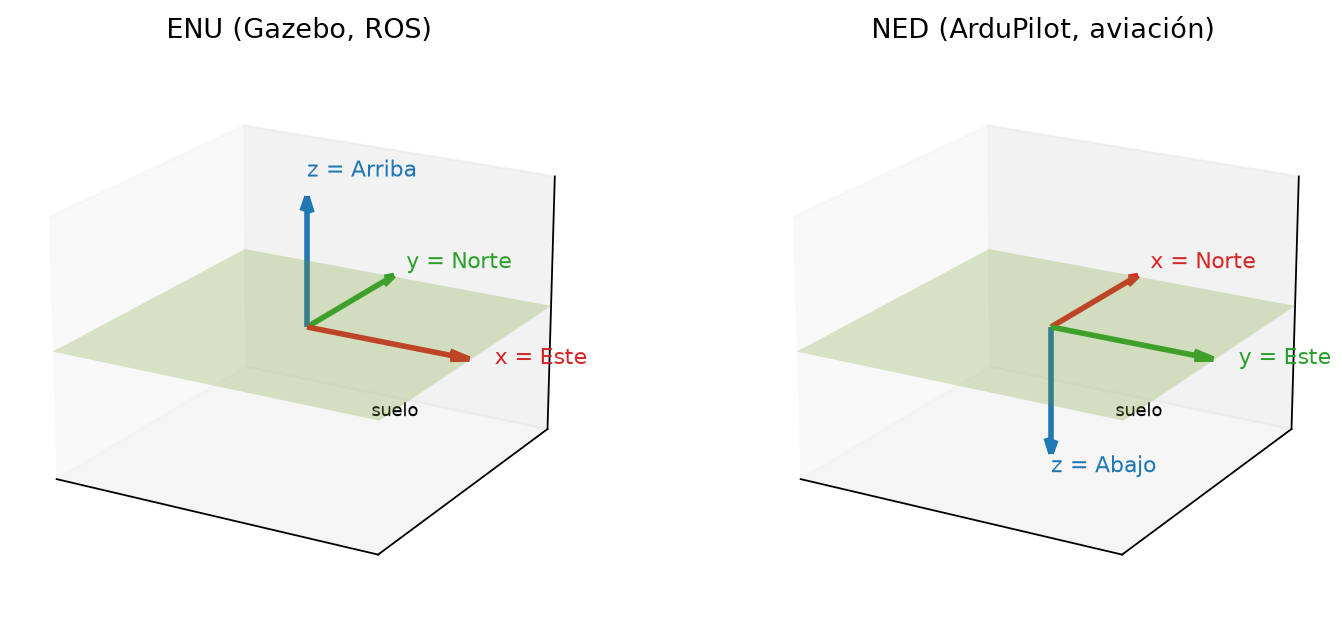
\includegraphics[width=0.9\textwidth]{c_marcos.png}
\caption{Los dos marcos del mundo. Confundirlos es una de las causas más comunes de errores en
drones.}
\end{figure}

\begin{figure}[H]
\centering
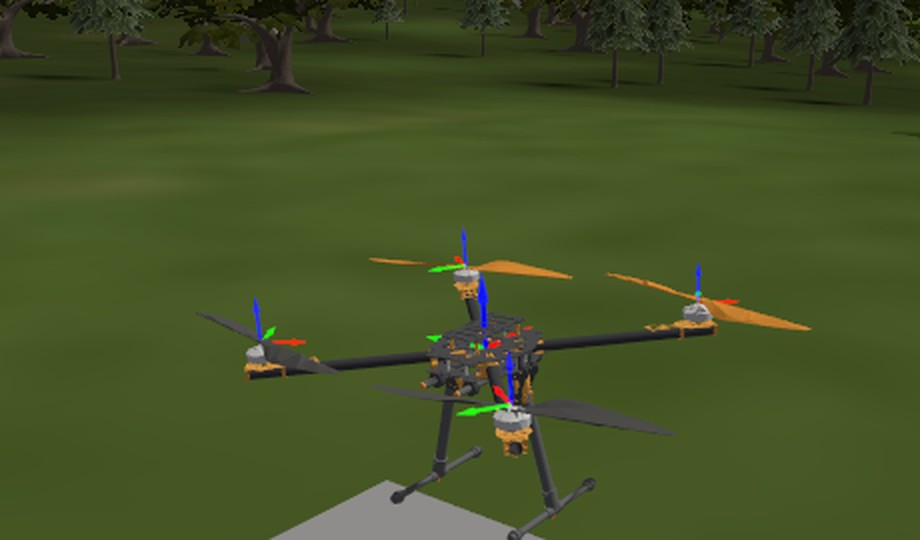
\includegraphics[width=0.6\textwidth]{gz_tarot_marcos.jpg}
\caption{En Gazebo se pueden mostrar los marcos de cada pieza del dron (rojo = \emph{x},
verde = \emph{y}, azul = \emph{z}).}
\end{figure}

\begin{leccion}
Durante el desarrollo, el vuelo con ArduPilot mandaba al dron 330~m lejos de donde debía ir: se
restaba dos veces la posición de salida al pasar del marco del mundo al marco local de ArduPilot. El
dron llegó a estrellarse contra un cerro. Se arregló midiendo el desfase entre los dos marcos en
lugar de suponerlo (sección~\ref{sec:plugin-ap}). Moraleja: \textbf{siempre verifica en qué marco
está cada número}.
\end{leccion}

\section{Rotaciones y ángulos de Euler}

La orientación del dron se puede describir con tres ángulos, alabeo $\phi$, cabeceo $\theta$ y
guiñada $\psi$ (los \textbf{ángulos de Euler}), aplicados en cierto orden. Para hacer cuentas es más
cómodo una \textbf{matriz de rotación} $R$ de $3\times3$: sus tres columnas son los ejes del dron
vistos desde el mundo. Multiplicar un vector del cuerpo por $R$ lo ``pasa'' al mundo. Por ejemplo,
la dirección del empuje es la tercera columna de $R$, $R e_3$.

\begin{tecnico}
Gazebo y ROS entregan la orientación como un \textbf{cuaternión} $(q_x, q_y, q_z, q_w)$: cuatro
números que representan una rotación sin las singularidades de los ángulos de Euler (que fallan
cuando el cabeceo llega a 90°). El código convierte cuaterniones a matrices con
\cod{dinamica.quat_a_rot}.
\end{tecnico}

\section{Las ecuaciones del dron en una página}

\begin{tcolorbox}[colback=white,colframe=NavyBlue!60!black,title=Modelo del cuadrirrotor]
\begin{align*}
\text{posición:}\quad & m\ddot p = T R e_3 - mg\,e_3 + d(t)\\
\text{orientación:}\quad & \dot R = R\hat\omega\\
\text{giro:}\quad & J\dot\omega = \tau - \omega\times J\omega\\
\text{motores:}\quad & f_i = k_f\omega_i^2,\qquad T = \textstyle\sum_i f_i,\qquad
\tau = \big(\textstyle\sum y_i f_i,\ -\sum x_i f_i,\ -\sum s_i k_m f_i\big)
\end{align*}
\end{tcolorbox}

No hace falta resolverlas a mano: Gazebo las integra por nosotros (Capítulo~\ref{cap:simulacion}).
Pero el controlador las usa para saber cuánto empuje y cuánto par pedir.
